% ma489_final_presentation.tex
\documentclass{beamer}

\usepackage{tikz,tkz-euclide}
\usetikzlibrary{arrows,decorations.pathmorphing,decorations.markings,backgrounds,positioning,fit,petri,patterns,calc,intersections}
\usetkzobj{all}
\usepackage{multicol}
\usepackage{color}
\usepackage{wasysym}

\usetheme{Warsaw}
\useoutertheme{infolines}
\beamertemplatenavigationsymbolsempty

\def \blue{\textcolor{blue}}
\def \brown{\textcolor{brown}}
\def \cyan{\textcolor{cyan}}
\def \green{\textcolor{green}}
\def \magenta{\textcolor{magenta}}
\def \orange{\textcolor{orange}}
\def \purple{\textcolor{purple}}
\def \red{\textcolor{red}}
\def \violet{\textcolor{violet}}
\def \yellow{\textcolor{yellow}}
\def \white{\textcolor{white}}

\synctex=1

\begin{document}
%titlepage info
\title[RK Methods with Rooted Trees]{Runge-Kutta Methods with Rooted Trees}
\subtitle[final presentation]{Final Presentation}
\author[R. Douglas]{\begin{tabular}{l r}
\textit{Author:} Richard Douglas & \textit{Supervisor:} Dr. Shengda Hu
\end{tabular}}
\institute[WLU MA489]{
  MA489 Research Seminar at Wilfrid Laurier University
}
\date[March 2014]{March 13, 2014}

\begin{frame}
  \titlepage
\end{frame}

%for when I arrive at a new section
\AtBeginSection[]{
  \begin{frame}
    \frametitle{Outline}
    \tableofcontents[currentsection]
  \end{frame}
}

\section[Rooted Tree Basics]{The Basics of Rooted Trees}

\begin{frame}{Rooted Trees Definition}
  \begin{definition}
  A \textbf{rooted tree} is a connected graph with directed edges and a finite number of vertices such that
  \begin{itemize}
  \item there is one vertex designated as the \textbf{root},
  \item every vertex except the root has exactly one parent, that is, if a vertex is not the root then 
           there is exactly one edge directed at it.
  \end{itemize}
  \end{definition}
  \textbf{Example:}
  \begin{center}
	 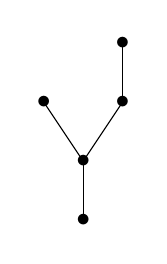
\begin{tikzpicture}[baseline=0cm]
	\node at (0,0)  {$\bullet$};
	\node at (0,0.75)  {$\bullet$};
	\node at (-0.5,1.5) {$\bullet$};
	\node at (0.5,1.5) {$\bullet$};
	\node at (0.5, 2.25) {$\bullet$};
	\draw (0,0)--(0,0.75);
	\draw (0,0.75)--(-0.5,1.5);
	\draw (0,0.75)--(0.5,1.5);
	\draw (0.5,1.5)--(0.5,2.25);
	\end{tikzpicture}
  \end{center}
  Vertices that are not the parent of any other vertices are called \textbf{leaves}.
\end{frame}

\begin{frame}{Rooted Trees Drawing Convention}
  Throughout this presentation the following convention is used:
  \begin{itemize}
  \item vertices are drawn without labels,
  \item the root is drawn at the bottom,
  \item child vertices are drawn above their respective parent vertex.
  \end{itemize}
  \white{.} \newline

  \begin{multicols}{3}
  \begin{center}
	 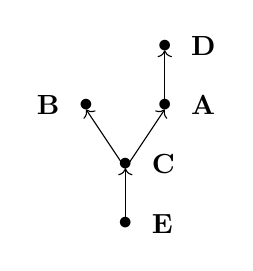
\begin{tikzpicture}[baseline=-0.25cm]
	\node at (0,0) [label=right:{$\mathbf{E}$}] {$\bullet$};
	\node at (0,0.75) [label=right:{$\mathbf{C}$}] {$\bullet$};
	\node at (-0.5,1.5)[label=left:{$\mathbf{B}$}] {$\bullet$};
	\node at (0.5,1.5)[label=right:{$\mathbf{A}$}] {$\bullet$};
	\node at (0.5, 2.25)[label=right:{$\mathbf{D}$}] {$\bullet$};
	\draw[arrows=->] (0,0)--(0,0.7);
	\draw[arrows=->] (0,0.7)--(-0.5,1.45);
	\draw[arrows=->] (0,0.7)--(0.5,1.45);
	\draw[arrows=->] (0.5,1.45)--(0.5,2.2);
	\end{tikzpicture}
  \end{center}
  \columnbreak
  \topskip0pt
  \vspace*{\fill}
     %\hfill $\mathbf{\longrightarrow}$ \hfill
     \hfill is drawn as \hfill
  \vspace*{\fill}
  \columnbreak
   \begin{center}
	 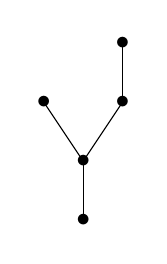
\begin{tikzpicture}[baseline=0cm]
	\node at (0,0)  {$\bullet$};
	\node at (0,0.75)  {$\bullet$};
	\node at (-0.5,1.5) {$\bullet$};
	\node at (0.5,1.5) {$\bullet$};
	\node at (0.5, 2.25) {$\bullet$};
	\draw (0,0)--(0,0.75);
	\draw (0,0.75)--(-0.5,1.5);
	\draw (0,0.75)--(0.5,1.5);
	\draw (0.5,1.5)--(0.5,2.25);
	\end{tikzpicture}
  \end{center}
  \end{multicols}
\end{frame}

\begin{frame}{Abstract Rooted Trees}
	 Two rooted trees are regarded as being \textbf{equivalent} if there exists an
	 order isomorphism between their vertex sets, that is, a bijection that preserves 
	 edge relations. \newline
	  
	  \noindent \textbf{Example:}
	   \begin{center}
		 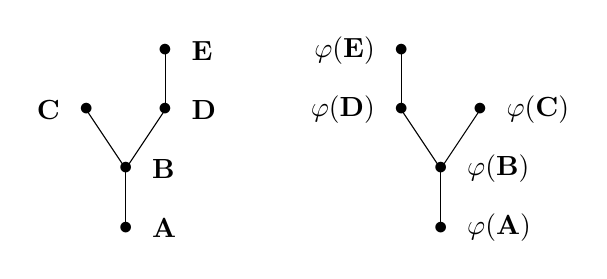
\begin{tikzpicture}[baseline=-0.25cm]
		\node at (0,0)[label=right:{$\mathbf{A}$}]  {$\bullet$};
		\node at (0,0.75)[label=right:{$\mathbf{B}$}]  {$\bullet$};
		\node at (-0.5,1.5)[label=left:{$\mathbf{C}$}] {$\bullet$};
		\node at (0.5,1.5)[label=right:{$\mathbf{D}$}] {$\bullet$};
		\node at (0.5, 2.25)[label=right:{$\mathbf{E}$}] {$\bullet$};
		\node at (4, 0)[label=right:{$\varphi(\mathbf{A})$}] {$\bullet$};
		\node at (4,0.75)[label=right:{$\varphi(\mathbf{B})$}]  {$\bullet$};
		\node at (3.5,1.5)[label=left:{$\varphi(\mathbf{D})$}] {$\bullet$};
		\node at (4.5,1.5)[label=right:{$\varphi(\mathbf{C})$}] {$\bullet$};
		\node at (3.5, 2.25)[label=left:{$\varphi(\mathbf{E})$}] {$\bullet$};
		\draw (0,0)--(0,0.75);
		\draw (0,0.75)--(-0.5,1.5);
		\draw (0,0.75)--(0.5,1.5);
		\draw (0.5,1.5)--(0.5,2.25);
		\draw (4,0)--(4,0.75);
		\draw (4,0.75)--(3.5,1.5);
		\draw (4,0.75)--(4.5,1.5);
		\draw (3.5,1.5)--(3.5,2.25);
		\end{tikzpicture}
	  \end{center}
%	  More explicitly, two rooted trees with respective vertex sets $V$, $V'$ and edge sets $E$, $E'$ are equivalent if 
%  	 $$\exists \mbox{ a bijection } \varphi:V \to V' \mbox{ such that } (a,b) \in E \iff (\varphi(a), \varphi(b)) \in E'$$
\end{frame}

\begin{frame}{Abstract Rooted Trees (cont.)}
  Thus each rooted tree belongs to a unique equivalence class with respect to this notion of equivalence. \newline
  
  \begin{itemize}
  \item For a given rooted tree, its \textbf{abstract rooted tree} is its equivalence class. \newline
  
  \item The letter \textbf{t} is used to denote an arbitrary rooted tree and 
  $|$\textbf{t}$|$ denotes the corresponding abstract rooted tree. \newline
  
  \item The set of all rooted trees is denoted \textbf{T}.
  \end{itemize}
\end{frame}

\begin{frame}{Important Functions on Trees}
  For a given rooted tree \textbf{t}, the following values are of interest:
  \begin{itemize}
    \item $r(t)$: the \textbf{order} or number of vertices in the tree,
    \item $\sigma(t)$: the \textbf{symmetry} or the number of automorphisms 
    			  for the tree, (that is, the number of bijections from the tree's vertex set
    		            to itself that preserve the ordering scheme,)  
    \item $\gamma(t)$: the \textbf{density} of the tree,
    			    (this is defined to be the value obtained by taking the order
			     of each subtree that would be formed if each vertex of the tree
			    were the root (not counting the vertices not at or above the
			    vertex) and then multiplying all of these values together.) 
  \end{itemize}
  \begin{center}
	 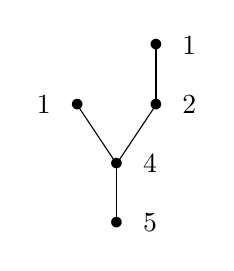
\begin{tikzpicture}[baseline=-0.25cm]
	\node at (0,0)[label=right:{$5$}]  {$\bullet$};
	\node at (0,0.75)[label=right:{$4$}]  {$\bullet$};
	\node at (-0.5,1.5)[label=left:{$1$}] {$\bullet$};
	\node at (0.5,1.5)[label=right:{$2$}] {$\bullet$};
	\node at (0.5, 2.25)[label=right:{$1$}] {$\bullet$};
	\draw (0,0)--(0,0.75);
	\draw (0,0.75)--(-0.5,1.5);
	\draw (0,0.75)--(0.5,1.5);
	\draw (0.5,1.5)--(0.5,2.25);
	\end{tikzpicture}
  \end{center}
\end{frame}

\begin{frame}{Important Functions on Trees (examples)}
  \begin{multicols}{2}
  \begin{center}
	 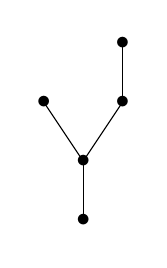
\begin{tikzpicture}[baseline=-0.25cm]
	\node at (0,0)  {$\bullet$};
	\node at (0,0.75)  {$\bullet$};
	\node at (-0.5,1.5) {$\bullet$};
	\node at (0.5,1.5) {$\bullet$};
	\node at (0.5, 2.25) {$\bullet$};
	\draw (0,0)--(0,0.75);
	\draw (0,0.75)--(-0.5,1.5);
	\draw (0,0.75)--(0.5,1.5);
	\draw (0.5,1.5)--(0.5,2.25);
	\end{tikzpicture}
  \end{center}
  \hfill$r(t) = 5, \sigma(t) = 1, \gamma(t) = 40$\hfill
  \columnbreak
  \begin{center}
	 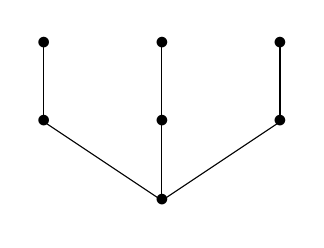
\begin{tikzpicture}[baseline=-0.25cm]
	\node at (0,0)  {$\bullet$};
	\node at (0,1)  {$\bullet$};
	\node at (-1.5,1) {$\bullet$};
	\node at (1.5,1) {$\bullet$};
	\node at (-1.5,2) {$\bullet$};
	\node at (0,2) {$\bullet$};
	\node at (1.5,2) {$\bullet$};
	\draw (0,0)--(0,1);
	\draw (0,0)--(-1.5,1);
	\draw (0,0)--(1.5,1);
	\draw (-1.5,1)--(-1.5,2);
	\draw (0,1)--(0,2);
	\draw (1.5,1)--(1.5,2);
	\end{tikzpicture}
  \end{center}
  \hfill $r(t) = 7, \sigma(t) = 6, \gamma(t) = 56$ \hfill
  \end{multicols}
\end{frame}

\begin{frame}{More Functions on Trees}
    $$ \alpha(t) := \frac{r(t)!}{\sigma(t)\gamma(t)} (= \frac{\beta(t)}{\gamma(t)})$$
    $$ \beta(t) := \frac{r(t)!}{\sigma(t)}$$
    \begin{itemize}
    \item $\alpha(t)$: the number of ways to label $\mathbf t$'s vertices using elements from the set
    	  $\{1,2, \dots, r(t)\}$ such that \newline
             \begin{enumerate}
             \item[1.] each vertex receives exactly one label (repetition is not allowed,) \newline
             \item[2.] labelings that indicate an automorphism are counted only once, \newline
             \item[3.] if $(a,b)$ is a directed edge in t's edge set, then the label for 
             $a$ is less than the label for $b$. \newline
             \end{enumerate}
    \item $\beta(t)$: same as $\alpha(t)$ but without the third condition. 
  \end{itemize}
\end{frame}  

\begin{frame}{What Condition 2. Means}
Condition 2. states that the following are counted as the same labeling:
 \begin{multicols}{2}
  \begin{center}
	 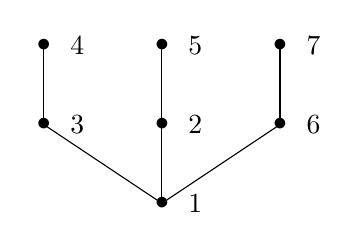
\begin{tikzpicture}[baseline=-0.25cm]
	\node at (0,0)[label=right:{$1$}]  {$\bullet$};
	\node at (0,1)[label=right:{$2$}]  {$\bullet$};
	\node at (-1.5,1)[label=right:{$3$}] {$\bullet$};
	\node at (1.5,1)[label=right:{$6$}] {$\bullet$};
	\node at (-1.5,2)[label=right:{$4$}] {$\bullet$};
	\node at (0,2)[label=right:{$5$}] {$\bullet$};
	\node at (1.5,2)[label=right:{$7$}] {$\bullet$};
	\draw (0,0)--(0,1);
	\draw (0,0)--(-1.5,1);
	\draw (0,0)--(1.5,1);
	\draw (-1.5,1)--(-1.5,2);
	\draw (0,1)--(0,2);
	\draw (1.5,1)--(1.5,2);
	\end{tikzpicture}
  \end{center}
  \columnbreak
  \begin{center}
	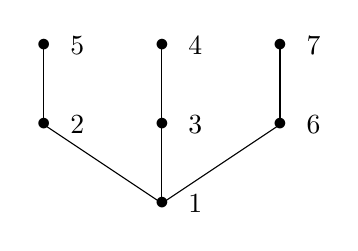
\begin{tikzpicture}[baseline=-0.25cm]
	\node at (0,0)[label=right:{$1$}]  {$\bullet$};
	\node at (0,1)[label=right:{$3$}]  {$\bullet$};
	\node at (-1.5,1)[label=right:{$2$}] {$\bullet$};
	\node at (1.5,1)[label=right:{$6$}] {$\bullet$};
	\node at (-1.5,2)[label=right:{$5$}] {$\bullet$};
	\node at (0,2)[label=right:{$4$}] {$\bullet$};
	\node at (1.5,2)[label=right:{$7$}] {$\bullet$};
	\draw (0,0)--(0,1);
	\draw (0,0)--(-1.5,1);
	\draw (0,0)--(1.5,1);
	\draw (-1.5,1)--(-1.5,2);
	\draw (0,1)--(0,2);
	\draw (1.5,1)--(1.5,2);
	\end{tikzpicture}
  \end{center}
  \end{multicols}
\end{frame}

\begin{frame}{Examples for $\alpha(t)$, $\beta(t)$}
  \begin{multicols}{2}
   \textbf{Tree:} 
   
  \textbf{$\alpha$ Labelings:}
  \end{multicols}
  \begin{multicols}{2}
   \begin{center}
	 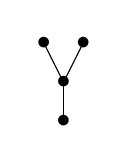
\begin{tikzpicture}[baseline=0cm]
	\node at (0,0)  {$\bullet$};
	\node at (0,0.5)  {$\bullet$};
	\node at (-0.25,1) {$\bullet$};
	\node at (0.25,1) {$\bullet$};
	\draw (0,0)--(0,0.5);
	\draw (0,0.5)--(-0.25,1);
	\draw (0,0.5)--(0.25,1);
	\end{tikzpicture}
  \end{center}
  
  \begin{center}
	 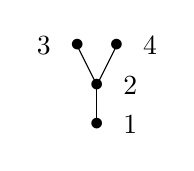
\begin{tikzpicture}[baseline=0cm]
	\node at (0,0)[label=right:{$1$}]  {$\bullet$};
	\node at (0,0.5)[label=right:{$2$}]  {$\bullet$};
	\node at (-0.25,1)[label=left:{$3$}] {$\bullet$};
	\node at (0.25,1)[label=right:{$4$}] {$\bullet$};
	\draw (0,0)--(0,0.5);
	\draw (0,0.5)--(-0.25,1);
	\draw (0,0.5)--(0.25,1);
	\end{tikzpicture}
  \end{center}
  \end{multicols}
  
  \textbf{$\beta$ Labelings:}
  \begin{multicols}{6}
  \begin{center}
	 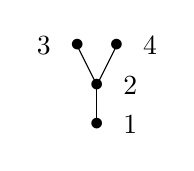
\begin{tikzpicture}[baseline=0cm]
	\node at (0,0)[label=right:{$1$}]  {$\bullet$};
	\node at (0,0.5)[label=right:{$2$}]  {$\bullet$};
	\node at (-0.25,1)[label=left:{$3$}] {$\bullet$};
	\node at (0.25,1)[label=right:{$4$}] {$\bullet$};
	\draw (0,0)--(0,0.5);
	\draw (0,0.5)--(-0.25,1);
	\draw (0,0.5)--(0.25,1);
	\end{tikzpicture}
  \end{center}
  
   \begin{center}
	 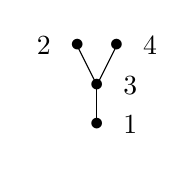
\begin{tikzpicture}[baseline=0cm]
	\node at (0,0)[label=right:{$1$}]  {$\bullet$};
	\node at (0,0.5)[label=right:{$3$}]  {$\bullet$};
	\node at (-0.25,1)[label=left:{$2$}] {$\bullet$};
	\node at (0.25,1)[label=right:{$4$}] {$\bullet$};
	\draw (0,0)--(0,0.5);
	\draw (0,0.5)--(-0.25,1);
	\draw (0,0.5)--(0.25,1);
	\end{tikzpicture}
  \end{center}
  
    \begin{center}
	 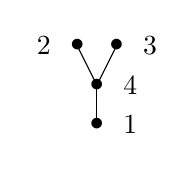
\begin{tikzpicture}[baseline=0cm]
	\node at (0,0)[label=right:{$1$}]  {$\bullet$};
	\node at (0,0.5)[label=right:{$4$}]  {$\bullet$};
	\node at (-0.25,1)[label=left:{$2$}] {$\bullet$};
	\node at (0.25,1)[label=right:{$3$}] {$\bullet$};
	\draw (0,0)--(0,0.5);
	\draw (0,0.5)--(-0.25,1);
	\draw (0,0.5)--(0.25,1);
	\end{tikzpicture}
  \end{center}
  
   \begin{center}
	 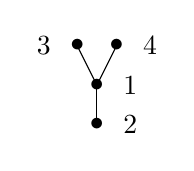
\begin{tikzpicture}[baseline=0cm]
	\node at (0,0)[label=right:{$2$}]  {$\bullet$};
	\node at (0,0.5)[label=right:{$1$}]  {$\bullet$};
	\node at (-0.25,1)[label=left:{$3$}] {$\bullet$};
	\node at (0.25,1)[label=right:{$4$}] {$\bullet$};
	\draw (0,0)--(0,0.5);
	\draw (0,0.5)--(-0.25,1);
	\draw (0,0.5)--(0.25,1);
	\end{tikzpicture}
  \end{center}
  
     \begin{center}
	 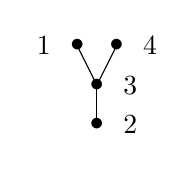
\begin{tikzpicture}[baseline=0cm]
	\node at (0,0)[label=right:{$2$}]  {$\bullet$};
	\node at (0,0.5)[label=right:{$3$}]  {$\bullet$};
	\node at (-0.25,1)[label=left:{$1$}] {$\bullet$};
	\node at (0.25,1)[label=right:{$4$}] {$\bullet$};
	\draw (0,0)--(0,0.5);
	\draw (0,0.5)--(-0.25,1);
	\draw (0,0.5)--(0.25,1);
	\end{tikzpicture}
  \end{center}
  
     \begin{center}
	 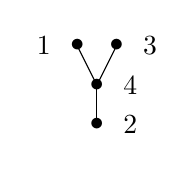
\begin{tikzpicture}[baseline=0cm]
	\node at (0,0)[label=right:{$2$}]  {$\bullet$};
	\node at (0,0.5)[label=right:{$4$}]  {$\bullet$};
	\node at (-0.25,1)[label=left:{$1$}] {$\bullet$};
	\node at (0.25,1)[label=right:{$3$}] {$\bullet$};
	\draw (0,0)--(0,0.5);
	\draw (0,0.5)--(-0.25,1);
	\draw (0,0.5)--(0.25,1);
	\end{tikzpicture}
  \end{center}
  \end{multicols}
  \begin{multicols}{6}
  \begin{center}
	 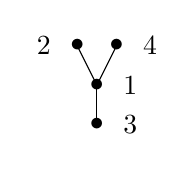
\begin{tikzpicture}[baseline=0cm]
	\node at (0,0)[label=right:{$3$}]  {$\bullet$};
	\node at (0,0.5)[label=right:{$1$}]  {$\bullet$};
	\node at (-0.25,1)[label=left:{$2$}] {$\bullet$};
	\node at (0.25,1)[label=right:{$4$}] {$\bullet$};
	\draw (0,0)--(0,0.5);
	\draw (0,0.5)--(-0.25,1);
	\draw (0,0.5)--(0.25,1);
	\end{tikzpicture}
  \end{center}

  \begin{center}
	 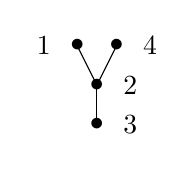
\begin{tikzpicture}[baseline=0cm]
	\node at (0,0)[label=right:{$3$}]  {$\bullet$};
	\node at (0,0.5)[label=right:{$2$}]  {$\bullet$};
	\node at (-0.25,1)[label=left:{$1$}] {$\bullet$};
	\node at (0.25,1)[label=right:{$4$}] {$\bullet$};
	\draw (0,0)--(0,0.5);
	\draw (0,0.5)--(-0.25,1);
	\draw (0,0.5)--(0.25,1);
	\end{tikzpicture}
  \end{center}

  \begin{center}
	 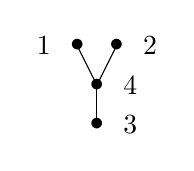
\begin{tikzpicture}[baseline=0cm]
	\node at (0,0)[label=right:{$3$}]  {$\bullet$};
	\node at (0,0.5)[label=right:{$4$}]  {$\bullet$};
	\node at (-0.25,1)[label=left:{$1$}] {$\bullet$};
	\node at (0.25,1)[label=right:{$2$}] {$\bullet$};
	\draw (0,0)--(0,0.5);
	\draw (0,0.5)--(-0.25,1);
	\draw (0,0.5)--(0.25,1);
	\end{tikzpicture}
  \end{center}

  \begin{center}
	 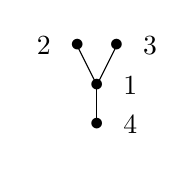
\begin{tikzpicture}[baseline=0cm]
	\node at (0,0)[label=right:{$4$}]  {$\bullet$};
	\node at (0,0.5)[label=right:{$1$}]  {$\bullet$};
	\node at (-0.25,1)[label=left:{$2$}] {$\bullet$};
	\node at (0.25,1)[label=right:{$3$}] {$\bullet$};
	\draw (0,0)--(0,0.5);
	\draw (0,0.5)--(-0.25,1);
	\draw (0,0.5)--(0.25,1);
	\end{tikzpicture}
  \end{center}
  
  \begin{center}
	 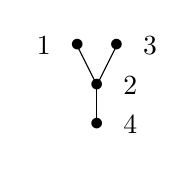
\begin{tikzpicture}[baseline=0cm]
	\node at (0,0)[label=right:{$4$}]  {$\bullet$};
	\node at (0,0.5)[label=right:{$2$}]  {$\bullet$};
	\node at (-0.25,1)[label=left:{$1$}] {$\bullet$};
	\node at (0.25,1)[label=right:{$3$}] {$\bullet$};
	\draw (0,0)--(0,0.5);
	\draw (0,0.5)--(-0.25,1);
	\draw (0,0.5)--(0.25,1);
	\end{tikzpicture}
  \end{center}
   
  \begin{center}
	 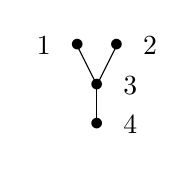
\begin{tikzpicture}[baseline=0cm]
	\node at (0,0)[label=right:{$4$}]  {$\bullet$};
	\node at (0,0.5)[label=right:{$3$}]  {$\bullet$};
	\node at (-0.25,1)[label=left:{$1$}] {$\bullet$};
	\node at (0.25,1)[label=right:{$2$}] {$\bullet$};
	\draw (0,0)--(0,0.5);
	\draw (0,0.5)--(-0.25,1);
	\draw (0,0.5)--(0.25,1);
	\end{tikzpicture}
  \end{center}
  \end{multicols}
\end{frame}

\begin{frame}{Notation for Rooted Trees}
  A rooted tree with a single vertex, that is, a tree with a root vertex and nothing else, is denoted by $\tau$.
  \begin{center}
	 \begin{tikzpicture}[baseline=0cm]
	\node at (0,0)  {$\bullet$};
	\end{tikzpicture}
  \end{center}
  Other rooted trees are denoted using a recursive notation. In general,
  $$\left[ t_1, t_2, \dots, t_m \right]$$
  denotes a rooted tree where the root has $m$ child nodes which form the respective subtrees $t_1, t_2, \dots, t_m$. 
  \newline
  
  Since a subtree can show up more than once, it is convenient to use powers in the notation to indicate repetition. 
  An arbitrary rooted tree can also be represented as
  $$\left[ t^{m_1}_1, t^{m_2}_2, \dots, t^{m_n}_n \right]$$
\end{frame}

\begin{frame}{Notation for Rooted Trees (examples)}
  \begin{multicols}{2}
  \begin{center}
  	\begin{tikzpicture}[baseline=0cm]
	\node at (0,0)  {$\bullet$};
	\node at (0,1)  {$\bullet$};
	\draw (0,0)--(0,1);
	\end{tikzpicture}
  \end{center}
  
  \begin{center}
  	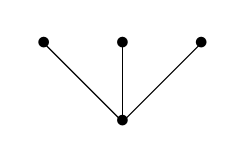
\begin{tikzpicture}[baseline=0cm]
	\node at (0,0)  {$\bullet$};
	\node at (-1,1) {$\bullet$};
	\node at (0,1)  {$\bullet$};
	\node at (1,1) {$\bullet$};
	\draw (0,0)--(-1,1);
	\draw (0,0)--(0,1);
	\draw (0,0)--(1,1);
	\end{tikzpicture}
  \end{center}
  \end{multicols}
  
  \begin{multicols}{2}
  \begin{center}
    $\left[ \tau \right]$
    \end{center}
    
    \begin{center}
    $\left[ \tau^3 \right]$
    \end{center}
  \end{multicols}
  \phantom{nothing}
  
  \begin{multicols}{2}
    \begin{center}
  	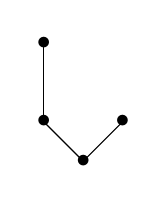
\begin{tikzpicture}[baseline=0.25cm]
	\node at (0,0)  {$\bullet$};
	\node at (-0.5,0.5)  {$\bullet$};
	\node at (0.5,0.5)  {$\bullet$};
	\node at (-0.5,1.5)  {$\bullet$};
	\draw (0,0)--(-0.5,0.5);
	\draw (0,0)--(0.5,0.5);
	\draw (-0.5,0.5)--(-0.5,1.5);
	\end{tikzpicture}
  \end{center}
  
   \begin{center}
  	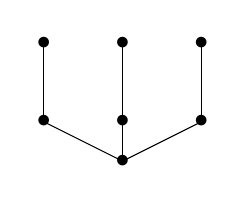
\begin{tikzpicture}[baseline=0.25cm]
	\node at (0,0)  {$\bullet$};
	\node at (-1,0.5)  {$\bullet$};
	\node at (0,0.5)  {$\bullet$};
	\node at (1,0.5)  {$\bullet$};
	\node at (-1,1.5)  {$\bullet$};
	\node at (0,1.5)  {$\bullet$};
	\node at (1,1.5)  {$\bullet$};
	\draw (0,0)--(-1,0.5);
	\draw (0,0)--(0,0.5);
	\draw (0,0)--(1,0.5);
	\draw (-1,0.5)--(-1,1.5);
	\draw (0,0.5)--(0,1.5);
	\draw (1,0.5)--(1,1.5);
	\end{tikzpicture}
  \end{center}
  \end{multicols}
  
  \begin{multicols}{2}
  \begin{center}
    $\left[ \left[ \tau \right] \tau \right]$
    \end{center}
    
    \begin{center}
    $\left[ \left[\tau\right]^3 \right]$
    \end{center}
  \end{multicols}
\end{frame}

\begin{frame}{Some Basic Results}
  \begin{theorem}
  Let \textbf{t} = $\left[ t^{m_1}_1, t^{m_2}_2, \dots, t^{m_n}_n \right]$ be a rooted tree, then
  \begin{enumerate}
    \item[1.] $r(t) = 1 + \sum_{i = 1}^{n}{m_ir(t_i)}$
    \item[2.] $\sigma(t) = \prod_{i = 1}^{n}{m_i!\sigma(t_i)^{m_i}}$
    \item[3.] $\gamma(t) = r(t)\prod_{i = 1}^{n}{\gamma(t_i)^{m_i}}$
    \end{enumerate}
    Also recall that
    \begin{enumerate}
    \item[4.] $\alpha(t) = \frac{r(t)!}{\sigma(t)\gamma(t)}$
    \item[5.] $\beta(t) = \frac{r(t)!}{\sigma(t)}$
    \end{enumerate}
  \end{theorem}
\end{frame}

\begin{frame}{Numerical Analysis with Rooted Trees}
Now that we know a bit about rooted trees and their properties, we can use them to solve
our problem in numerical analysis, that is, \newline

\textit{``How can we derive the system of equations for Runge-Kutta
methods of a desired order without having to take so many Taylor expansions?''} \newline

We will see that both the Taylor expansion
$$y(x_n+h) = y(x_n) + hy'(x_n) + \frac{h^2}{2!}y''(x_n) + \dots$$
and the Runge-Kutta approximation
$$y_{n + 1} = y_n + b_1hf(Y_1) + b_2hf(Y_2) + \dots + b_shf(Y_s)$$
can be expressed in terms of rooted trees. 

\end{frame}

\section[Rooted Trees Taylor Expansion]{Using Rooted Trees to get the Taylor Expansion}

\begin{frame}{The Elementary Differential}
Assume that we have an autonomous ordinary differential equation, that is
$$y'(x) = f(y(x)) \mbox{ for all } x \in \left[a,b\right], \mbox{ and } y(x_0) = y_0.$$
(Note that $y(x)$ can be an ordinary function or a vector.)
\begin{definition}
Given a tree \textbf{t} and a function $f:R^N \to R^N$ analytic in some neighbourhood of $y$,
the \textbf{Elementary Differential} $F(t)(y)$ is defined recursively by
$$F(\tau)(y) = f(y)$$
$$F(\left[t_1, t_2, \dots, t_m \right])(y) = f^{(m)}(y)(F(t_1)(y),F(t_2)(y), \dots, F(t_m)(y))$$
\end{definition}
\end{frame}

\begin{frame}{The Elementary Differential (examples)}
\begin{multicols}{2}
  \begin{center}
    \begin{tikzpicture}[baseline=-0.25cm]
       \node at (0,-1)[label=right:{$f$}]  {$\bullet$};
     \end{tikzpicture}
  \end{center}
  
  \begin{center}
  	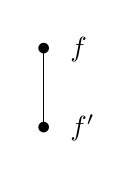
\begin{tikzpicture}[baseline=-0.25cm]
	\node at (0,0)[label=right:{$f'$}]  {$\bullet$};
	\node at (0,1)[label=right:{$f$}]  {$\bullet$};
	\draw (0,0)--(0,1);
	\end{tikzpicture}
  \end{center}
\end{multicols}
Note that $\frac{d}{dx}f(y(x)) = f'(y(x))f(y(x))$.
\begin{multicols}{2}
    \begin{center}
  	\begin{tikzpicture}[baseline=-0.25cm]
	\node at (0,-2)[label=right:{$f''$}]  {$\bullet$};
	\node at (-1,-1)[label=right:{$f$}]  {$\bullet$};
	\node at (1,-1)[label=right:{$f$}]  {$\bullet$};
	\draw (0,-2)--(-1,-1);
	\draw (0,-2)--(1,-1);
	\end{tikzpicture}
  \end{center}

  \begin{center}
    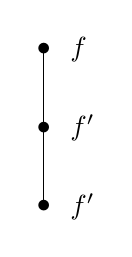
\begin{tikzpicture}[baseline=-0.25cm]
       \node at (0,0)[label=right:{$f$}]  {$\bullet$};
       \node at (0,-1)[label=right:{$f'$}]  {$\bullet$};
       \node at (0,-2)[label=right:{$f'$}]  {$\bullet$};
       \draw (0,-2)--(0,-1);
       \draw (0,-1)--(0,0);
     \end{tikzpicture}
  \end{center}
\end{multicols}
Similarly, $\frac{d^2}{dx^2}f(y(x)) = F(\left[\tau^2\right])(y(x)) + F(\left[\left[\tau\right]\right])(y(x))$.

\end{frame}

\begin{frame}{Taking the Derivative of an Elementary Differential}
\begin{lemma}
Let \textbf{t} be a rooted tree, then
$$\frac{d}{dx}F(|t|)(y)$$
is the sum of $F(u)(y)$ over all rooted trees \textbf{u} such that if a leaf vertex is removed from \textbf{u},
it becomes \textbf{t}.
\end{lemma}
\pause
\textbf{Sketch Proof:}

 This can be proved by complete induction on the order of \textbf{t} (on $n = r(t)$).
 A key step is in how if we let $\textbf{t} = \left[t_1, t_2, \dots t_m\right]$, then
 $$\frac{d}{dx}F(|t|)(y(x)) = \frac{d}{dx} (f^{(m)}(y)(F(t_1)(y),F(t_2)(y), \dots, F(t_m)(y)))$$
 The extended product rule can then be used. The $f^{(m+1)}(y)$ term corresponds to adding
 a leaf to the root. The rest of the terms follow from the inductive hypothesis.
\end{frame}

\begin{frame}{Taking the Derivative of an Elementary Differential (cont.)}
An important thing to note about the lemma is that it is actually the location
of the inserted leaf vertex that is summed over. It does not matter if two different locations
of the inserted leaf result in trees that are equivalent.
\begin{center}
  	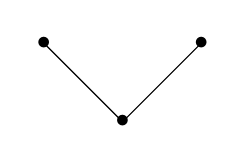
\begin{tikzpicture}[baseline=0cm]
	\node at (0,0)  {$\bullet$};
	\node at (-1,1)  {$\bullet$};
	\node at (1,1)  {$\bullet$};
	\draw (0,0)--(-1,1);
	\draw (0,0)--(1,1);
	\end{tikzpicture}
  \end{center}
  $$F(\left[\tau^2\right])(y(x)) = f''(y(x))f(y(x))^2$$
  \begin{multicols}{3}
   \pause
   \begin{center}
  	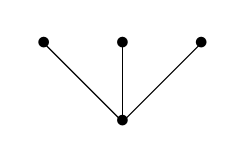
\begin{tikzpicture}[baseline=0cm]
	\node at (0,0)  {$\bullet$};
	\node at (-1,1)  {$\bullet$};
	\node at (0,1)  {$\bullet$};
	\node at (1,1)  {$\bullet$};
	\draw (0,0)--(-1,1);
	\draw (0,0)--(0,1);
	\draw (0,0)--(1,1);
	\end{tikzpicture}
  \end{center}
  \pause
  \begin{center}
  	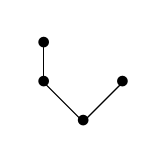
\begin{tikzpicture}[baseline=0cm]
	\node at (0,0)  {$\bullet$};
	\node at (-0.5,0.5)  {$\bullet$};
	\node at (0.5,0.5)  {$\bullet$};
	\node at (-0.5,1)  {$\bullet$};
	\draw (0,0)--(-0.5,0.5);
	\draw (0,0)--(0.5,0.5);
	\draw (-0.5,0.5)--(-0.5,1);
	\end{tikzpicture}
  \end{center}
  
\begin{center}
  	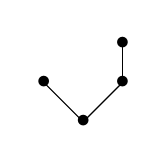
\begin{tikzpicture}[baseline=0cm]
	\node at (0,0)  {$\bullet$};
	\node at (-0.5,0.5)  {$\bullet$};
	\node at (0.5,0.5)  {$\bullet$};
	\node at (0.5,1)  {$\bullet$};
	\draw (0,0)--(-0.5,0.5);
	\draw (0,0)--(0.5,0.5);
	\draw (0.5,0.5)--(0.5,1);
	\end{tikzpicture}
  \end{center}
  \end{multicols}
  \pause
  $$\frac{d}{dx}F(\left[\tau^2\right])(y(x)) = F(\left[\tau^3\right])(y(x)) + 2 F(\left[\left[\tau\right]\tau\right])(y(x))$$
\end{frame}

\begin{frame}{Obtaining Derivatives for the Taylor expansion}
\begin{theorem}
Let $y(x)$ be a function such that $y'(x) = f(y(x))$, then assuming that it exists,
$$y^{(k)}(x) = \sum_{r(|t|) = k}{\alpha(|t|)F(|t|)(y(x))}$$
That is, the $k^{th}$ derivative of $y$ can be found using a representative of each equivalence class from
the set all rooted trees with $k$ vertices.
\end{theorem}
\pause
\textbf{Sketch Proof:}

By applying the preceding lemma repeatedly, it is clear that we will be summing all rooted trees of order $k$, 
however some rooted trees will be appearing more than once. This is where $\alpha(t)$ comes into play. \newline

An alternative way to interpret $\alpha(t)$ is as the number of orders in which you ``can add vertices 
to the top'' so that $|\mathbf{t}|$ is constructed.
\end{frame}

\begin{frame}{Obtaining the Taylor Expansion}
\begin{theorem}
The Taylor expansion of $y(x)$ about $x = x_n$ (assuming it exists) is
$$y(x_n + h) = y(x_n) + \sum_{|t| \in T}{\frac{h^{r(|t|)}}{\sigma(|t|)\gamma(|t|)}F(|t|)(y(x_n))}$$ 
\end{theorem}
\pause
\textbf{Proof:}
$$y(x_n + h) = y(x_n) + \sum_{k = 1}^{\infty}{\frac{h^k}{k!}y^{(k)}(x_n)} = 
 y(x_n) + \sum_{k = 1}^{\infty}{\frac{h^k}{k!} \sum_{r(|t|) = k}{\alpha(|t|)F(|t|)(y(x_n))}}$$
 $$= y(x_n) + \sum_{|t| \in T}{\frac{h^{r(|t|)}\alpha(|t|)}{r(|t|)!}F(|t|)(y(x_n))}$$
 Recalling that $\alpha(t) = \frac{r(t)!}{\sigma(t)\gamma(t)}$, the result follows.
\end{frame}

\begin{frame}{Obtaining the Taylor Expansion (cont.)}
\begin{corollary}
For any natural number $P$, 
$$y(x_n + h) = y(x_n) + \sum_{r(|t|) \le P}{\red{\frac{1}{\gamma(|t|)}}
\frac{h^{r(|t|)}}{\sigma(|t|)}F(|t|)(y(x_n))} + O(h^{P+1})$$
\end{corollary}
This gives us the truncated Taylor expansion of the exact solution to the ODE in terms of rooted trees.
\end{frame}

\section[Rooted Trees RK Approximation]{Using Rooted Trees to get the Runge-Kutta Approximation}
\begin{frame}{A Brief Recap of Runge-Kutta}
\begin{center}
 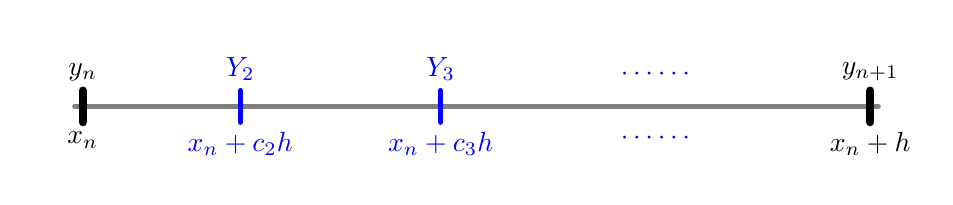
\begin{tikzpicture}%[scale=0.9]
  \tkzInit[xmax=11, ymax=1.5]\tkzClip[space=0.2]
  \begin{scope}[xshift=5.5cm,yshift=0.7cm]
   \tkzDefPoints{-5/0/xn, 5/0/xn1, -5/0.2/u, -5/-0.2/b}
   \tkzDefBarycentricPoint(xn=.8,xn1=.2) \tkzGetPoint{a2}
   \tkzDefBarycentricPoint(xn=.6,xn1=.5) \tkzGetPoint{a3}
   \tkzDefBarycentricPoint(a3=.5,xn1=.5) \tkzGetPoint{m}
   \tkzDefPointsBy[translation= from xn to a2](u,b){u2,b2}
   \tkzDefPointsBy[translation= from xn to a3](u,b){u3,b3}
   \tkzDefPointsBy[translation= from xn to xn1](u,b){un1,bn1}
   \tkzDefPointsBy[translation= from xn to m](u,b){um,bm}
   \tkzDrawPoints[fill,color=black](xn,xn1,u,b,un1,bn1)
   \tkzDrawLine[line width=2pt, color=gray, add=0.01 and 0.01](xn,xn1)
   \tkzDrawSegments[line width=3pt, color=black](u,b un1,bn1)
   \tkzDrawSegments[line width=2pt, color=blue](u2,b2 u3,b3)
   \tkzLabelPoint[above](u){$y_n$}
   \tkzLabelPoint[above,color=blue](u2){$Y_2$}
   \tkzLabelPoint[above,color=blue](u3){$Y_3$}
   \tkzLabelPoint[above,color=blue](um){$\cdots \cdots$}
   \tkzLabelPoint[above](un1){$y_{n+1}$}
   \tkzLabelPoint[below](b){$x_n$}
   \tkzLabelPoint[below,color=blue](b2){$x_n + c_2 h$}
   \tkzLabelPoint[below,color=blue](b3){$x_n + c_3 h$}
   \tkzLabelPoint[below,color=blue](bm){$\cdots \cdots$}
   \tkzLabelPoint[below](bn1){$x_n + h$}
  \end{scope}
 \end{tikzpicture}
\end{center}
For an explicit Runge-Kutta method with $s$ stages we need to determine
$$X_1 = x_n, X_2 = x_n + \mathbf{c_2}h, X_3 = x_n + \mathbf{c_3}h, \dots, X_s = x_n + \mathbf{c_s}h$$
We also need to know how each stage depends on the previously computed stage derivatives.
$$Y_1 = y_n, Y_2 = y_n + \mathbf{a_{21}}hf(Y_1), \dots, Y_s = y_n + \sum_{j = 1}^{s-1}{\mathbf{a_{sj}}hf(Y_j)}$$
Lastly we need to know the weights
$$y_{n + 1} = y_n + \mathbf{b_1}hf(Y_1) + \mathbf{b_2}hf(Y_2) + \dots \mathbf{b_s}hf(Y_s)$$
\end{frame}

\begin{frame}{The Weight Functions}
\begin{definition}
Let
\noindent
\begin{center}
\begin{tabular}{r | l}
$c$ & $A$ \\ 
\hline 
  & $b$
\end{tabular}
\end{center}
denote the tableau for an explicit Runge-Kutta method with $s$ stages.
\pause
Then the \textbf{elementary weights} $\Phi(t)$, \textbf{internal weights} $\Phi_i(t)$,
and \textbf{derivative weights} $\Phi_i^D(t)$ for $t \in T$ and $i = 1, 2, \dots, s$
are defined by
\begin{multicols}{2}
\begin{center}
$\Phi(t) = \sum_{i = 1}^s{b_i\Phi_i^D(t)},$
\end{center} 
\columnbreak
\begin{center}
$\Phi_i(t) = \sum_{j = 1}^{i - 1}{a_{ij}\Phi_j^D(t)},$
\end{center}
\end{multicols}
$$\Phi_i^D(t) = \left\{ 
 \begin{array}{ll}
 1 & : t = \tau \\
 \prod_{j = 1}^m{\Phi_i(t_j)} & : t = \left[t_1, t_2, \dots, t_m \right]
 \end{array}
 \right.$$
\end{definition}
\end{frame}

\begin{frame}{Weights and Internal Weights look the same}
$$\Phi_i(t) = \sum_{j = 1}^{i - 1}{a_{ij}\Phi_j^D(t)}
\mbox{ comes from }
Y_i = y_n + \sum_{j = 1}^{i - 1}{a_{ij}hf(Y_j)},$$
and
$$\Phi(t) = \sum_{i = 1}^s{b_i\Phi_i^D(t)}
\mbox{ comes from }
y_{n+1} = y_n + \sum_{i = 1}^{s}{b_ihf(Y_i)}.$$
What's interesting to note is that the approximation for $y(x_n + h)$ is computed in a way that is
similar to the way that stages are computed. The calculation for $y_{n + 1}$ can be thought of as 
a final stage.
\end{frame}

\begin{frame}{Where the Derivative Weights come from}
The motivation for the derivative weights comes from the following result:
\begin{lemma}
The Taylor expansion for
$$hf\left(y_n + \sum_{|t| \in T}{\purple{\Phi_i(|t|)}\frac{h^{r(|t|)}}{\sigma(|t|)}F(|t|)(y_n) }\right)$$
is
$$\sum_{|t| \in T}{\purple{\Phi_i^D(|t|)}\frac{h^{r(|t|)}}{\sigma(|t|)}F(|t|)(y_n) }$$
\end{lemma}

The proof of this result is not appropriate for a short presentation as there will be many things 
going on at once. If you are interested, we can talk about it afterwards.
\end{frame}

\begin{frame}{The Taylor Expansion for the Runge-Kutta Approximation}
\begin{theorem}
The truncated Taylor expansions for the stages, stage derivatives, and approximation 
for an explicit s-stage Runge-Kutta method of order $P$ are
$$Y_i = y_n + \sum_{r(|t|) \le P}\purple{\Phi_i(|t|)} {\frac{h^{r(|t|)}}{\sigma(|t|)}F(|t|)(y_n)} + O(h^{P + 1}),$$
$$hf(Y_i) = \sum_{r(|t|) \le P}{\purple{\Phi_i^D(|t|)}\frac{h^{r(|t|)}}{\sigma(|t|)}F(|t|)(y_n) } + O(h^{P + 1}),$$
\hfill (where $i = 1, 2, \dots, s$)
$$y_{n + 1} =  y_n + \sum_{r(|t|) \le P}{\red{\Phi(|t|)}\frac{h^{r(|t|)}}{\sigma(|t|)}F(|t|)(y_n)} + O(h^{P + 1})$$
\end{theorem}
\end{frame}

\begin{frame}{The Taylor Expansion for the Runge-Kutta Approximation (proof)}
\textbf{Proof:}

The proof is by complete induction on the stage number.
$$\Phi_1(t) = 0 \mbox{ for all } t \in T \Longrightarrow Y_1 = y_n$$
$$\Phi_1^D(t) = \left\{ 
	\begin{array}{l l}
	1 & : t = \tau \\
	0 & : otherwise
	\end{array}
\right.
\Longrightarrow
hf(Y_1) = \frac{h^{r(|\tau|)}}{\sigma(|\tau|)}f(y_n)$$ \newline
The base case clearly holds.
\end{frame}

\begin{frame}{The Taylor Expansion for the Runge-Kutta Approximation (proof cont.)}
Suppose that for all $1 \le i \le k$, the result holds, that is
$$Y_i = y_n + \sum_{r(|t|) \le P}{\purple{\Phi_i(|t|)}\frac{h^{r(|t|)}}{\sigma(|t|)}F(|t|)(y_n)} + O(h^{P + 1}),$$
then applying the most recent lemma gives us (for all $1 \le i \le k$)
$$hf(Y_i) = \sum_{r(|t|) \le P}{\purple{\Phi_i^D(|t|)}\frac{h^{r(|t|)}}{\sigma(|t|)}F(|t|)(y_n) } + O(h^{P + 1}).$$
\end{frame}
\begin{frame}{The Taylor Expansion for the Runge-Kutta Approximation (proof cont.)}
The next stage is computed as follows
$$Y_{k + 1} = y_n + \sum_{j = 1}^k{a_{(k+1)j}hf(Y_j)}$$ 
$$= y_n + \sum_{r(|t|) \le P}{\sum_{j = 1}^k{\purple{a_{(k+1)j}} {\purple{\Phi_j^D(|t|)} \frac{h^{r(|t|)}}
{\sigma(|t|)}F(|t|)(y_n) } }} + O(h^{P + 1})$$
$$= y_n + \sum_{r(|t|) \le P}{\red{\Phi_{k + 1}(|t|)} \frac{h^{r(|t|)}}{\sigma(|t|)}F(|t|)(y_n)} + O(h^{P + 1})$$
Thus the inductive hypothesis holds. The expansion for $y_{n + 1}$ is just a special case where the $a_{ij}$ terms
are replaced by $b_i$. By induction, we have our result.
\end{frame}

\section[Deriving the Methods]{Deriving Runge-Kutta Methods with Rooted Trees}

\begin{frame}{Equating the Expansions}
Assume that we have an autonomous ordinary differential equation,
$$y'(x) = f(y(x)) \mbox{ for all } x \in \left[a,b\right], y(x_0) = y_0$$
An $s$-stage order $P$ Runge-Kutta method will require the terms of the truncated Taylor expansion for the exact solution
$$y(x_n + h) \approx y(x_n) + \sum_{r(|t|) \le P}\red{\frac{1}{\gamma(|t|)}}{\frac{h^{r(|t|)}}{\sigma(|t|)}F(|t|)(y(x_n))}$$
to equate with the terms of the truncated Taylor expansion for the approximation
$$y_{n + 1} = y_n + \sum_{r(|t|) \le P}{\red{\Phi(|t|)} \frac{h^{r(|t|)}}{\sigma(|t|)}F(|t|)(y_n)}.$$

\end{frame}

\begin{frame}{Equating the Expansions (cont.)}
This is accomplished if
$$\red{\Phi(|t|) = \frac{1}{\gamma(|t|)}} \mbox{ for all } |t| \mbox{ such that } r(|t|) \le P$$
In other words, the equations that the $a_{ij}$, $b_i$, and $c_j$ terms must satisfy can be obtained 
without doing any Taylor expansions! \newline

Instead, we can take a representative of each equivalence class from the set of rooted trees with order $\le P$
and equate $\Phi(|t|) = \frac{1}{\gamma(|t|)}$ for each one.
\end{frame}

\begin{frame}{An Easier Way to Compute $\Phi(|t|)$}
\begin{itemize}
\item At the root write $b_i$ in the sum. Label the root with the letter $i$. 
\begin{multicols}{2}
\begin{center}
  	\begin{tikzpicture}[baseline=0cm]
	\node at (0,0)[label=right:{i}]  {$\bullet$};
	\end{tikzpicture}
  \end{center}
  
  $b_i$
  \end{multicols}

\item At leaf vertices write $c_*$ in the sum where $*$ is the label of the leaf's parent.
\begin{multicols}{2}
\begin{center}
  	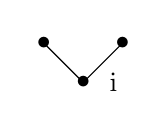
\begin{tikzpicture}[baseline=0cm]
	\node at (0,0)[label=right:{i}]  {$\bullet$};
	\node at (-0.5,0.5) {$\bullet$};
	\node at (0.5,0.5) {$\bullet$};
	\draw (0,0)--(-0.5,0.5);
	\draw (0,0)--(0.5,0.5);
	\end{tikzpicture}
  \end{center}
  
  $b_ic_ic_i$
  \end{multicols}

\item At all other vertices write  $a_{*-}$ in the sum where $*$ is the label of the vertex's parent and $-$ is a letter not
yet used as a label. \linebreak Label the vertex with $-$.
\begin{multicols}{2}
 \begin{center}
  	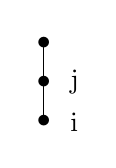
\begin{tikzpicture}[baseline=0cm]
	\node at (0,0)[label=right:{i}]  {$\bullet$};
	\node at (0,0.5)[label=right:{j}]  {$\bullet$};
	\node at (0,1)  {$\bullet$};
	\draw (0,0)--(0,0.5);
	\draw (0,0.5)--(0,1);
	\end{tikzpicture}
  \end{center}
  
  $b_ia_{ij}c_j$
\end{multicols}
\end{itemize}
\end{frame}

\begin{frame}{Deriving the Third Order methods with 3 stages}
The rooted trees with order $\le 3$ and corresponding equations are
\begin{multicols}{2}
 \begin{center}
  	\begin{tikzpicture}[baseline=0cm]
	\node at (0,0)  {$\bullet$};
	\end{tikzpicture}
  \end{center}

 \begin{center}
  	\begin{tikzpicture}[baseline=0cm]
	\node at (0,0)  {$\bullet$};
	\node at (0,1)  {$\bullet$};
	\draw (0,0)--(0,1);
	\end{tikzpicture}
  \end{center}
\end{multicols}

\begin{multicols}{2}
\begin{center}
$\sum_{i = 1}^s{b_i} = 1$
\end{center}

\begin{center}
$\sum_{i = 1}^s{b_ic_i} = 1/2$
\end{center}
\end{multicols}

\begin{multicols}{2}
 \begin{center}
  	\begin{tikzpicture}[baseline=0cm]
	\node at (0,-1.5)  {$\bullet$};
	\node at (-1,-0.5) {$\bullet$};
	\node at (1,-0.5) {$\bullet$};
	\draw (0,-1.5)--(-1,-0.5);
	\draw (0,-1.5)--(1,-0.5);
	\end{tikzpicture}
  \end{center}

 \begin{center}
  	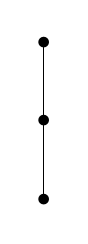
\begin{tikzpicture}[baseline=0cm]
	\node at (0,0)  {$\bullet$};
	\node at (0,1)  {$\bullet$};
	\node at (0,2)  {$\bullet$};
	\draw (0,0)--(0,1);
	\draw (0,1)--(0,2);
	\end{tikzpicture}
  \end{center}
\end{multicols}

\begin{multicols}{2}
\begin{center}
$\sum_{i = 1}^s{b_ic_i^2} = 1/3$
\end{center}

\begin{center}
$\sum_{i = 1}^s{\sum_{j = 1}^{i - 1}{b_ia_{ij}c_j}} = 1/6$
\end{center}
\end{multicols}

\end{frame}

\begin{frame}{Deriving the Third Order methods with 3 stages (cont.)}
We thus have the system of equations
$$b_1 + b_2 + b_3 = 1$$
$$b_2c_2 + b_3c_3 = 1/2$$
$$b_2c_2^2 + b_3c_3^2 = 1/3$$
$$b_3a_{32}c_2 = 1/6$$
We can now let $c_2$ and $c_3$ be free parameters
in order to make the first few equations into a linear system.
$$\left[ \begin{matrix}
1 & 1 & 1 \\
0 & c_2 & c_3 \\
0 & c_2^2 & c_3^2
\end{matrix} \right] 
\left[ \begin{matrix} 
b_1 \\ b_2 \\ b_3
\end{matrix} \right] = 
\left[ \begin{matrix} 
1 \\ 1/2 \\ 1/6
\end{matrix} \right]$$
and then deal with the fourth equation once $b_1, b_2, b_3$ are known.
\end{frame}

\begin{frame}{Deriving the Third Order methods with 3 stages (cont.)}
The determinant of the coefficient matrix in the linear system is 
$$c_2c_3(c_3 - c_2)$$
And the fourth equation was
$$b_3a_{32}c_2 = 1/6$$

There are three cases where a solution exists:
\begin{enumerate}
\item[1.] $c_2c_3(c_3 - c_2) \ne 0$
\item[2.] $c_2 = 2/3, c_3 = 0, b_3 \ne 0$
\item[3.] $c_2 = 2/3, c_3 = 2/3, b_3 \ne 0$
\end{enumerate}
\end{frame}

\section[Simplifying Conditions for Deriving Methods]{Simplifying Conditions for Deriving Methods of Higher Order}

\begin{frame}{The Motivation for Imposing Conditions}
$$\red{\Phi(|t|) = \frac{1}{\gamma(|t|)}} \mbox{ for all } |t| \mbox{ such that } r(|t|) \le P$$

Thus far we have figured out a way to obtain the system of equations without doing any Taylor expansions. \newline

However, as the order of the methods we wish to derive increases, so does the number of rooted trees. 
In fact, the number of rooted trees we must deal with seems to grow exponentially as the sought after order
increases. \newline

The idea now is to impose simplifying conditions that the coefficients need to satisfy so that we have to worry about
less rooted trees.
\end{frame}

\begin{frame}{The $B(\eta)$ Conditions}
The following rooted trees all have a similar form, that is, they all consist of only a root with leaves.
\begin{multicols}{4}
  \begin{center}
  	\begin{tikzpicture}[baseline=0cm]
	\node at (0,-1)  {$\bullet$};
	\end{tikzpicture}
  \end{center}
 
 \begin{center}
  	\begin{tikzpicture}[baseline=0cm]
	\node at (0,-1)  {$\bullet$};
	\node at (0,0)  {$\bullet$};
	\draw (0,-1)--(0,0);
	\end{tikzpicture}
  \end{center}
  
  \begin{center}
  	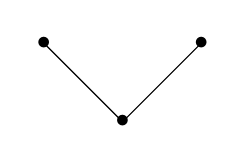
\begin{tikzpicture}[baseline=0cm]
	\node at (-1,0)  {$\bullet$};
	\node at (1,0)  {$\bullet$};
	\node at (0,-1)  {$\bullet$};
	\draw (0,-1)--(-1,0);
	\draw (0,-1)--(1,0);
	\end{tikzpicture}
  \end{center}
  
  \begin{center}
  	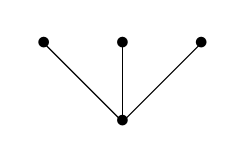
\begin{tikzpicture}[baseline=0cm]
	\node at (-1,0)  {$\bullet$};
	\node at (0,0)  {$\bullet$};
	\node at (1,0)  {$\bullet$};
	\node at (0,-1)  {$\bullet$};
	\draw (0,-1)--(-1,0);
	\draw (0,-1)--(0,0);
	\draw (0,-1)--(1,0);
	\end{tikzpicture}
  \end{center}
\end{multicols}
\white{.} \newline

For a Runge-Kutta method to have order $P$, we would normally have to worry about $P$ of these trees.
We can instead impose the condition
$$\sum_{i = 1}^s{b_ic_i^{k - 1}} = 1/k \mbox{ for all } k = 1, 2, \dots, \eta$$
and then set $\eta$ equal to $P$.
\end{frame}

\begin{frame}{The $D(1)$ Condition}
Suppose that we have the equations holding for two rooted trees of the following form
\begin{multicols}{2}
\begin{center}
  	\begin{tikzpicture}[baseline=0cm]
	\node at (0,0)  {$\bullet$};
	\node at (0,1)  {$*$};
	\draw (0,0)--(0,1);
	\end{tikzpicture}
  \end{center}
 
 \begin{center}
  	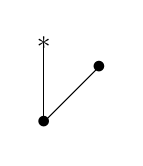
\begin{tikzpicture}[baseline=0cm]
	\node at (0,0)  {$\bullet$};
	\node at (0,1)  {$*$};
	\node at (0.7,0.7)  {$\bullet$};
	\draw (0,0)--(0,1);
	\draw (0,0)--(0.7,0.7);
	\end{tikzpicture}
  \end{center}
\end{multicols}
\pause
If the $D(1)$ condition holds, then the equation for the following tree is automatically satisfied
\begin{center}
  	\begin{tikzpicture}[baseline=0cm]
	\node at (0,0.7)  {$\bullet$};
	\node at (0,1.5)  {$*$};
	\node at (0,0)  {$\bullet$};
	\draw (0,0)--(0,0.7);
	\draw (0,0.7)--(0,1.5);
	\end{tikzpicture}
  \end{center}
\end{frame}

\begin{frame}{What the $D(1)$ Condition is}
\begin{multicols}{4}
\begin{center}
  	\begin{tikzpicture}[baseline=0cm]
	\node at (0,0)  {$\bullet$};
	\node at (0,1)  {$*$};
	\draw (0,0)--(0,1);
	\end{tikzpicture}
  \end{center}
 
 \begin{center}
  	\begin{tikzpicture}[baseline=0cm]
	\node at (0,0)  {$\bullet$};
	\node at (0,1)  {$*$};
	\node at (0.7,0.7)  {$\bullet$};
	\draw (0,0)--(0,1);
	\draw (0,0)--(0.7,0.7);
	\end{tikzpicture}
  \end{center}
  \columnbreak
  \topskip0pt
  \vspace*{\fill}
     \hfill $\Longrightarrow$ \hfill
  \vspace*{\fill}
  \columnbreak
 \begin{center}
  	\begin{tikzpicture}[baseline=0cm]
	\node at (0,0.7)  {$\bullet$};
	\node at (0,1.5)  {$*$};
	\node at (0,0)  {$\bullet$};
	\draw (0,0)--(0,0.7);
	\draw (0,0.7)--(0,1.5);
	\end{tikzpicture}
  \end{center}
\end{multicols}
Let's call these trees (from left to right) $\mathbf{t_1}, \mathbf{t_2}, \mathbf{t_3}$.
Then in general,
$$\frac{1}{\gamma(t_1)} - \frac{1}{\gamma(t_2)} = \frac{1}{\gamma(t_3)}$$
Thus we want to force
$$\sum_j{b_j*} - \sum_j{b_jc_j*} = \sum_j\sum_i{b_ia_{ij}*}$$
\end{frame}

\begin{frame}{What the $D(1)$ Condition is (cont.)}
The $D(1)$ condition states that 
$$b_j(1 - c_j) = \sum_{i = 1}^s{b_ia_{ij}} \mbox{ for any } j = 1, 2, \dots, s$$ \newline

\pause
In general, the $D(k)$ condition states that (for any $j = 1, 2, \dots, s$)
$$\frac{1}{q}b_j(1 - c_j^q) = \sum_{i = 1}^s{b_i c_i^{q - 1}a_{ij}} \mbox{ for all } q = 1,2, \dots, k$$
but for explicit Runge-Kutta methods, only the $D(1)$ condition can be used as the $D(2)$ condition leads
to an inconsistent system of equations.
\end{frame}

\begin{frame}{D(1) Condition Examples}
\begin{multicols}{4}
  \begin{center}
  	\begin{tikzpicture}[baseline=0cm]
	\node at (0,-0.75)  {$\bullet$};
	\node at (0,0)  {$\bullet$};
	\draw (0,-0.75)--(0,0);
	\end{tikzpicture}
  \end{center}
  \columnbreak
  \begin{center}
  	\begin{tikzpicture}[baseline=0cm]
	\node at (0,-0.75)  {$\bullet$};
	\node at (-0.75,0)  {$\bullet$};
	\node at (0.75,0)  {$\bullet$};
	\draw (0,-0.75)--(-0.75,0);
	\draw (0,-0.75)--(0.75,0);
	\end{tikzpicture}
  \end{center}
  \columnbreak
  \topskip0pt
  \vspace*{\fill}
     \hfill $\Longrightarrow$ \hfill
  \vspace*{\fill}
  \columnbreak
  \begin{center}
  	\begin{tikzpicture}[baseline=0cm]
	\node at (0,-0.75)  {$\bullet$};
	\node at (0,0)  {$\bullet$};
	\node at (0,0.75)  {$\bullet$};
	\draw (0,-0.75)--(0,0);
	\draw (0,0)--(0,0.75);
	\end{tikzpicture}
  \end{center}
\end{multicols}
\begin{multicols}{4}
\begin{center}
  	\begin{tikzpicture}[baseline=0cm]
	\node at (0,-0.75)  {$\bullet$};
	\node at (0,0)  {$\bullet$};
	\node at (0,0.75)  {$\bullet$};
	\draw (0,-0.75)--(0,0);
	\draw (0,0)--(0,0.75);
	\end{tikzpicture}
  \end{center}
  \columnbreak
 \begin{center}
  	\begin{tikzpicture}[baseline=0cm]
	\node at (0,-0.75)  {$\bullet$};
	\node at (-0.5,0)  {$\bullet$};
	\node at (0.5,0)  {$\bullet$};
	\node at (-0.5,0.75)  {$\bullet$};
	\draw (0,-0.75)--(-0.5,0);
	\draw (0,-0.75)--(0.5,0);
	\draw (-0.5,0)--(-0.5,0.75);
	\end{tikzpicture}
  \end{center}
  \columnbreak
  \topskip0pt
  \vspace*{\fill}
     \hfill $\Longrightarrow$ \hfill
  \vspace*{\fill}
  \columnbreak
  \begin{center}
  	\begin{tikzpicture}[baseline=0cm]
	\node at (0,-0.75)  {$\bullet$};
	\node at (0,0)  {$\bullet$};
	\node at (0,0.75)  {$\bullet$};
	\node at (0,1.5)  {$\bullet$};
	\draw (0,-0.75)--(0,0);
	\draw (0,0)--(0,0.75);
	\draw (0,0.75)--(0,1.5);
	\end{tikzpicture}
  \end{center}
\end{multicols}
\begin{multicols}{4}
  \begin{center}
  	\begin{tikzpicture}[baseline=0cm]
	\node at (0,-0.75)  {$\bullet$};
	\node at (-0.75,0)  {$\bullet$};
	\node at (0.75,0)  {$\bullet$};
	\draw (0,-0.75)--(-0.75,0);
	\draw (0,-0.75)--(0.75,0);
	\end{tikzpicture}
  \end{center}
  \columnbreak
  \begin{center}
  	\begin{tikzpicture}[baseline=0cm]
	\node at (0,-0.75)  {$\bullet$};
	\node at (-0.75,0)  {$\bullet$};
	\node at (0,0)  {$\bullet$};
	\node at (0.75,0)  {$\bullet$};
	\draw (0,-0.75)--(-0.75,0);
	\draw (0,-0.75)--(0,0);
	\draw (0,-0.75)--(0.75,0);
	\end{tikzpicture}
  \end{center}
  \columnbreak
   \topskip0pt
  \vspace*{\fill}
     \hfill $\Longrightarrow$ \hfill
  \vspace*{\fill}
  \columnbreak
  \begin{center}
  	\begin{tikzpicture}[baseline=0cm]
	\node at (0,-0.75)  {$\bullet$};
	\node at (0,0)  {$\bullet$};
	\node at (-0.5,0.75)  {$\bullet$};
	\node at (0.5,0.75)  {$\bullet$};
	\draw (0,-0.75)--(0,0);
	\draw (0,0)--(-0.5,0.75);
	\draw (0,0)--(0.5,0.75);
	\end{tikzpicture}
  \end{center}
\end{multicols}
\end{frame}

\begin{frame}{Deriving the Fourth Order methods with 4 stages}
The $B(4)$ condition takes care of
\begin{multicols}{4}
  \begin{center}
  	\begin{tikzpicture}[baseline=0cm]
	\node at (0,-0.6)  {$\bullet$};
	\end{tikzpicture}
  \end{center}
 
 \begin{center}
  	\begin{tikzpicture}[baseline=0cm]
	\node at (0,-0.6)  {$\bullet$};
	\node at (0,0)  {$\bullet$};
	\draw (0,-0.6)--(0,0);
	\end{tikzpicture}
  \end{center}
  
  \begin{center}
  	\begin{tikzpicture}[baseline=0cm]
	\node at (-0.6,0)  {$\bullet$};
	\node at (0.6,0)  {$\bullet$};
	\node at (0,-0.6)  {$\bullet$};
	\draw (0,-0.6)--(-0.6,0);
	\draw (0,-0.6)--(0.6,0);
	\end{tikzpicture}
  \end{center}
  
  \begin{center}
  	\begin{tikzpicture}[baseline=0cm]
	\node at (-0.6,0)  {$\bullet$};
	\node at (0,0)  {$\bullet$};
	\node at (0.6,0)  {$\bullet$};
	\node at (0,-0.6)  {$\bullet$};
	\draw (0,-0.6)--(-0.6,0);
	\draw (0,-0.6)--(0,0);
	\draw (0,-0.6)--(0.6,0);
	\end{tikzpicture}
  \end{center}
\end{multicols}
The $D(1)$ condition takes care of
\begin{multicols}{3}
\begin{center}
  	\begin{tikzpicture}[baseline=0cm]
	\node at (0,-1.6)  {$\bullet$};
	\node at (0,-0.8)  {$\bullet$};
	\node at (0,0)  {$\bullet$};
	\draw (0,-1.5)--(0,-0.8);
	\draw (0,-0.8)--(0,0);
	\end{tikzpicture}
  \end{center}
  
\begin{center}
  	\begin{tikzpicture}[baseline=0cm]
	\node at (0,-1.5)  {$\bullet$};
	\node at (0,-1.0)  {$\bullet$};
	\node at (0,-0.5)  {$\bullet$};
	\node at (0,0)  {$\bullet$};
	\draw (0,-1.5)--(0,-1.0);
	\draw (0,-1.0)--(0,-0.5);
	\draw (0,-0.5)--(0,0);
	\end{tikzpicture}
  \end{center}
  
  \begin{center}
  	\begin{tikzpicture}[baseline=0cm]
	\node at (0,-1.6)  {$\bullet$};
	\node at (0,-0.8)  {$\bullet$};
	\node at (-0.5,0)  {$\bullet$};
	\node at (0.5,0)  {$\bullet$};
	\draw (0,-1.6)--(0,-0.8);
	\draw (0,-0.8)--(-0.5,0);
	\draw (0,-0.8)--(0.5,0);
	\end{tikzpicture}
  \end{center}
\end{multicols}
What's left?
\begin{center}
  	\begin{tikzpicture}[baseline=0cm]
	\node at (0,-0.75)  {$\bullet$};
	\node at (-0.5,0)  {$\bullet$};
	\node at (0.5,0)  {$\bullet$};
	\node at (-0.5,0.75)  {$\bullet$};
	\draw (0,-0.75)--(-0.5,0);
	\draw (0,-0.75)--(0.5,0);
	\draw (-0.5,0)--(-0.5,0.75);
	\end{tikzpicture}
  \end{center}
\end{frame}

\begin{frame}{Deriving the Fourth Order methods with 4 stages (cont.)}
To deal with
\begin{multicols}{2}
\begin{center}
  	\begin{tikzpicture}[baseline=0cm]
	\node at (0,-0.75)  {$\bullet$};
	\node at (-0.5,0)  {$\bullet$};
	\node at (0.5,0)  {$\bullet$};
	\node at (-0.5,0.75)  {$\bullet$};
	\draw (0,-0.75)--(-0.5,0);
	\draw (0,-0.75)--(0.5,0);
	\draw (-0.5,0)--(-0.5,0.75);
	\end{tikzpicture}
  \end{center}
  
  $$\sum_{i = 1}^4\sum_{j = 1}^{i - 1}{b_ic_ia_{ij}c_j} = 1/8$$
\end{multicols}
\pause
we can subtract it from 
\begin{multicols}{2}
\begin{center}
  	\begin{tikzpicture}[baseline=0cm]
	\node at (0,-1.6)  {$\bullet$};
	\node at (0,-0.8)  {$\bullet$};
	\node at (0,0)  {$\bullet$};
	\draw (0,-1.5)--(0,-0.8);
	\draw (0,-0.8)--(0,0);
	\end{tikzpicture}
  \end{center}
  
  $$\sum_{i = 1}^4\sum_{j = 1}^{i - 1}{b_ia_{ij}c_j} = 1/6$$
\end{multicols}
\pause
To get the more convenient equation
$$\sum_{i = 1}^4\sum_{j = 1}^{i - 1}{b_i(1 - c_i)a_{ij}c_j} = b_3(1 - c_3)a_{32}c_2 = 1/24$$
\end{frame}

\begin{frame}{Deriving the Fourth Order methods with 4 stages (cont.)}
We thus have the system of equations
$$\sum_{i = 1}^4{b_ic_i^{k - 1}} = 1/k \mbox{ for all } k = 1, 2, \dots, 4$$
$$b_j(1 - c_j) = \sum_{i = 1}^4{b_ia_{ij}} \mbox{ for any } j = 1, 2, \dots, 4$$
$$b_3(1 - c_3)a_{32}c_2 = 1/24$$ \newline
\pause
A nice consequence of the $D(1)$ condition is that it immediately implies that $c_4 = 1$.
\end{frame}

\begin{frame}{Deriving the Fourth Order methods with 4 stages (cont.)}
A fourth order method with 4 stages can thus be constructed as follows:
\begin{itemize}
\pause \item Choose values for $c_2$ and $c_3$, noting that $c_1 = 0$ and $c_4 = 1$.
\pause \item Obtain $b_1, b_2, b_3, b_4$ by solving the linear system
$$\sum_{i = 1}^4{b_ic_i^{k - 1}} = 1/k \mbox{ for all } k = 1, 2, \dots, 4$$
\pause \item Set $a_{32} = \frac{1}{24b_3(1 - c_3)c_2}, a_{31} = c_3 - a_{32}, a_{21} = c_2$. 
\pause \item Obtain $a_{41}, a_{42}, a_{43}$ by using the $D(1)$ equations
$$a_{4j} = \frac{b_j(1 - c_j) - \sum_{i = 1}^{3}{b_ia_{ij}}}{b_4} \mbox{ for } j = 1, 2, 3$$
\end{itemize}
\pause
There are some subtleties but by following this approach, we can get our fourth order Runge-Kutta!
\end{frame}

\begin{frame}{Concluding Remarks}
Something that's interesting to note is that the approach of using rooted trees to derive
Runge-Kutta methods discussed in this presentation more or less applies to implicit 
Runge-Kutta methods as well. \newline

A reason why implicit methods may be of interest is because explicit Runge-Kutta methods 
can never be A-stable. \newline

If time permits, the final report may also include use of Runge-Kutta to aid in solving a problem related to Financial Math.
(That being computing the portfolios on the Efficient Frontier.) \newline

Thank you for viewing my presentation. \smiley{}
\end{frame}

\begin{frame}{How to Prove the Scary Lemma}
Remember this? \newline
\begin{lemma}
The Taylor expansion for
$$hf\left(y_n + \sum_{|t| \in T}{\purple{\Phi_i(|t|)}\frac{h^{r(|t|)}}{\sigma(|t|)}F(|t|)(y_n) }\right)$$
is
$$\sum_{|t| \in T}{\purple{\Phi_i^D(|t|)}\frac{h^{r(|t|)}}{\sigma(|t|)}F(|t|)(y_n) }$$
\end{lemma}
\white{.} \newline
Read on for instructions on how to prove it.
\end{frame}

\begin{frame}{How to Prove the Scary Lemma (cont.)}
We will need to use the following general result
\begin{theorem}
$$f(y + \sum_{i = 1}^m{\delta_i}) = \sum_{I \in I_m}{\frac{1}{\sigma(I)}f^{(\#I)}(y)}\delta_{I}$$
\end{theorem}
Where
\begin{itemize}
\item $I_m$ is the collection of finite sequences of the form $(i_1, i_2, \dots, i_n)$ 
where each term is of the set \{1,2, \dots, m\}. (The empty sequence $()$ is included.)
\item  $\delta_I = (\delta_{i_1}, \delta_{i_2}, \dots, \delta_{i_n})$ for $I = (i_1, i_2, \dots, i_n)$.  
\item $\sigma(I)$ is the number of ways of permuting the elements of the sequence without changing it.
$$\sigma(I) = k_1!k_2! \dots k_m!$$ 
where $k_j$ is the number of times $j$ appears in the sequence.
\end{itemize}
\end{frame}

\begin{frame}{How to Prove the Scary Lemma (cont.)}
The idea is that with the rooted trees, there is a finite number of trees of a given order 
so $T$ is a countably infinite set and we can write
$$T = \{t_1, t_2, t_3, \dots \}$$
The sequence $I = (i_1, i_2, \dots, i_n)$ will correspond with $(t_{i_1}, t_{i_2}, \dots t_{i_n})$.

This means 
$$\frac{1}{\sigma(I)}f^{(\#I)}(y)\delta_I = 
f^{(n)}(y)\frac{\Phi_i(t_{i_1})F(t_{i_1})(y) \Phi_i(t_{i_2})F(t_{i_2})(y) \dots \Phi_i(t_{i_n})F(t_{i_n})(y)}
{\sigma(I) \sigma(t_{i_1})\sigma(t_{i_2}) \dots \sigma(t_{i_n})}$$ 
$$= \frac{\Phi_i^D(\left[ t_{i_1}, t_{i_2}, \dots t_{i_n} \right])F(\left[ t_{i_1}, t_{i_2}, \dots t_{i_n} \right])(y)}
{\sigma(\left[ t_{i_1}, t_{i_2}, \dots t_{i_n} \right])}$$
The above is a sketch and does not show everything that is going on. It does not show the ${r(t_{i_j})}$
multiplying together to form $r(\left[ t_{i_1}, t_{i_2}, \dots t_{i_n} \right]) - 1$ and is for the general case
when $t \ne \tau$ ($\tau$ corresponds to $I = ()$ and is trivial.) 
\end{frame}

\end{document}